\chapter{Problem statement}

In this chapter, we describe in detail the optimization problem that we address in this thesis. This problem was originally assigned in the qualifying round of Google Hash Code 2021. Google Hash Code was a global team programming competition, running between 2014--2022, where teams of 2--4 competitors solved an optimization problem with the goal of achieving the best score in a limited time of 4 hours.

The standard solution procedure was as follows: Read the input data, create a trivial solution and write it to the output file in the specified format, and upload the solution to the evaluation system, where you could see not only the total score, but also some informative statistics, such as the number of cars that reached the finish before the deadline. For some datasets, an interactive visualization of the simulation process was also available, allowing to see the structure of a particular dataset. Although the local simulator was not needed to solve the problem, the manual upload of the solution to the evaluation system was slow and cumbersome and therefore not suitable for the use of efficient optimization algorithms.

Most teams were able to construct trivial solutions, which they then tried to improve by randomly changing the values. However, the best teams were able to write their own local simulator and use it to run multiple heuristics to get a better total score. Still, there was no time for anything more complex than a simple local search.

The total score is the sum of the scores of all 6 datasets \textbf{(a - f)}. The first dataset \textbf{(a)} serves as a "toy problem" mainly for debugging purposes, but the rest of the datasetes are large enough for the optimization. It should be noted that the distribution of points among the datasets is uneven, so the contestants mostly focused on the datasets with the highest possible score \textbf{(d, f)} and pragmatically skipped optimizing the rest \textbf{(b, c, e)}.

\section{Problem description}

The full problem statement\footnote{\url{https://github.com/google/coding-competitions-archive/blob/main/hashcode/hashcode_2021_qualification_round.pdf}} is available in the Google Coding Competitions archive~\cite{google_coding_competitions}. Here we describe only important details for the reader.
In short, the task is as follows: \textit{Given a city plan describing intersections and streets and cars with planned paths through the city, optimize the schedule of traffic lights to minimize the total amount of time spent in traffic, and help as many cars as possible reach their destination before a specified deadline.}

In terms of graph theory, the city plan is \textit{a directed graph}. The intersections are \textit{vertices} and the streets are \textit{directed edges} (See Figure~\ref{fig:hashcode_city_plan}). The planned path for each car is indeed a \textit{path} in this graph because it has a different start and end, and no intersection is repeated.

\begin{figure}
    \centering
    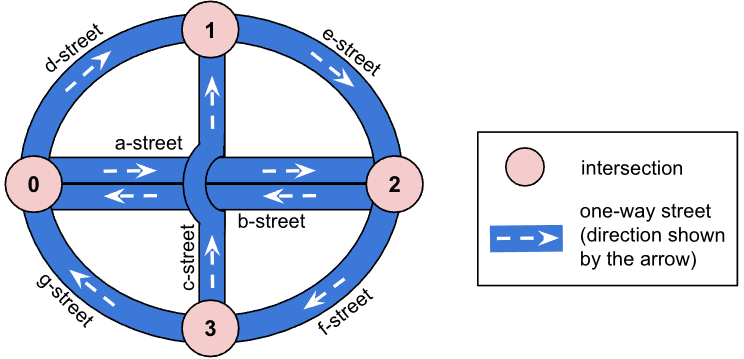
\includegraphics[width=\linewidth]{img/hashcode/figure1.png}
    %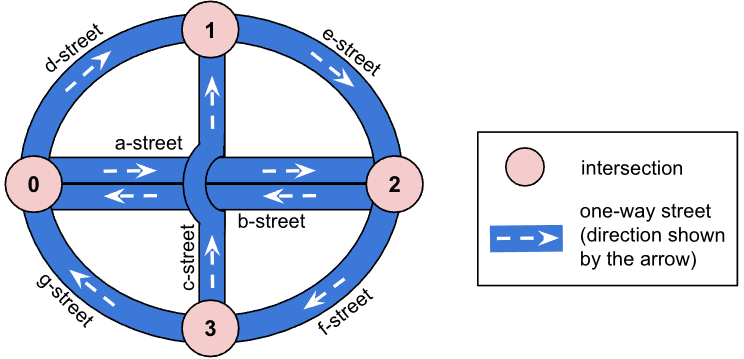
\includegraphics[width=.8\linewidth]{img/hashcode/figure1.png}
    \caption[Example of a city plan]{
        Example of a city plan \cite{google_coding_competitions}.
    }
    \label{fig:hashcode_city_plan}
\end{figure}

\subsection{Streets and intersections}
%\paragraph{Streets and intersections}

In the city, we have a set of intersections
$I$, where $2 \leq \abs{I} \leq 10^5$,
and a set of streets
$S \subseteq \{(u, v) | u,v \in I \land u \neq v\}$, where $2 \leq \abs{S} \leq 10^5$.
Each street $s \in S$ is a unique one-way connection between two different intersections $u$, $v$; two distinct streets in opposite directions between the same two intersections $(u, v)$, $(v, u)$ are allowed. Each street $s \in S$ has a fixed time $l(s) \in \mathbb{N}_+$ that it takes a car to get from the beginning to the end of the street, independently of the other cars on the street.
Each intersection $i \in I$ has a set of incoming streets $S_i^+ \subset S$, where $|S_i^+| \geq 1$, and a set of outgoing streets $S_i^- \subset S$, where $|S_i^-| \geq 1$; thus each intersection has at least one incoming street and at least one outgoing street.

\subsection{Traffic lights and schedules}

In each intersection $i \in I$, there is a traffic light at the end of each \textit{incoming} street $s^+ \in S_i^+$. The traffic light has two states --- green and red. Green means the cars from this street can pass through the intersection and continue to any \textit{outgoing} street $s^- \in S_i^-$ in their path. Red means the cars must stop until the light turns green again. At most one traffic light can be green at each intersection at any time.

When the light is red, cars arriving at the end of a street queue up and wait for the light to turn green. The queue does not take up any space and does not change the distance cars have to travel. When the light is green, one car can pass through an intersection every second. Passing through an intersection, i.e. moving from the end of an incoming street to the beginning of an outgoing street, takes no additional time.

For each intersection $i \in I$, we can set a traffic light schedule. This schedule determines the order and duration of green light for the incoming streets of the intersection. The schedule repeats in a cycle until the end of the simulation (See Figure~\ref{fig:hashcode_traffic_lights}). Each street can appear at most once in the schedule. If a street is not included in the schedule, it is red the whole time, and any waiting cars are blocked. By default, intersections have no schedule and all streets are red.

% https://tex.stackexchange.com/questions/69869/image-taking-up-full-page
\begin{figure}[ht] % h = here, t = top, p = page of floats
    \centering
    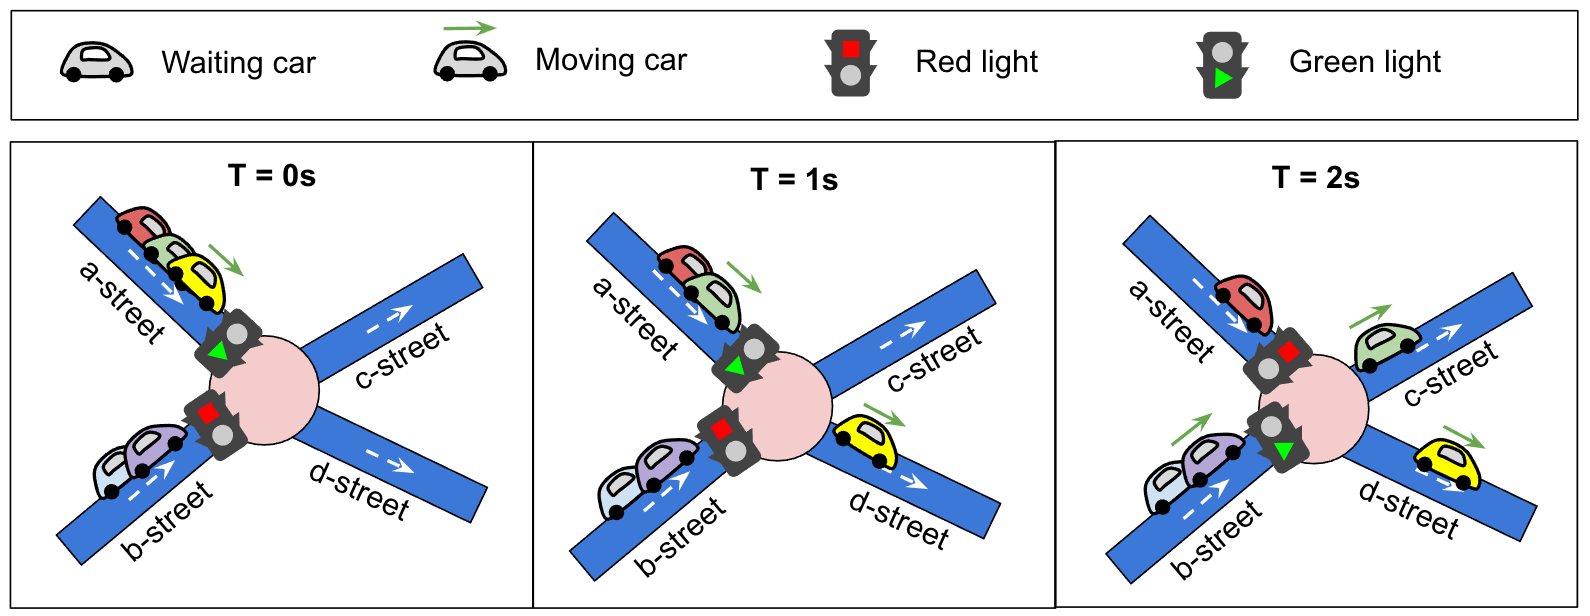
\includegraphics[width=\linewidth]{img/hashcode/figure2-abc.png}
    % 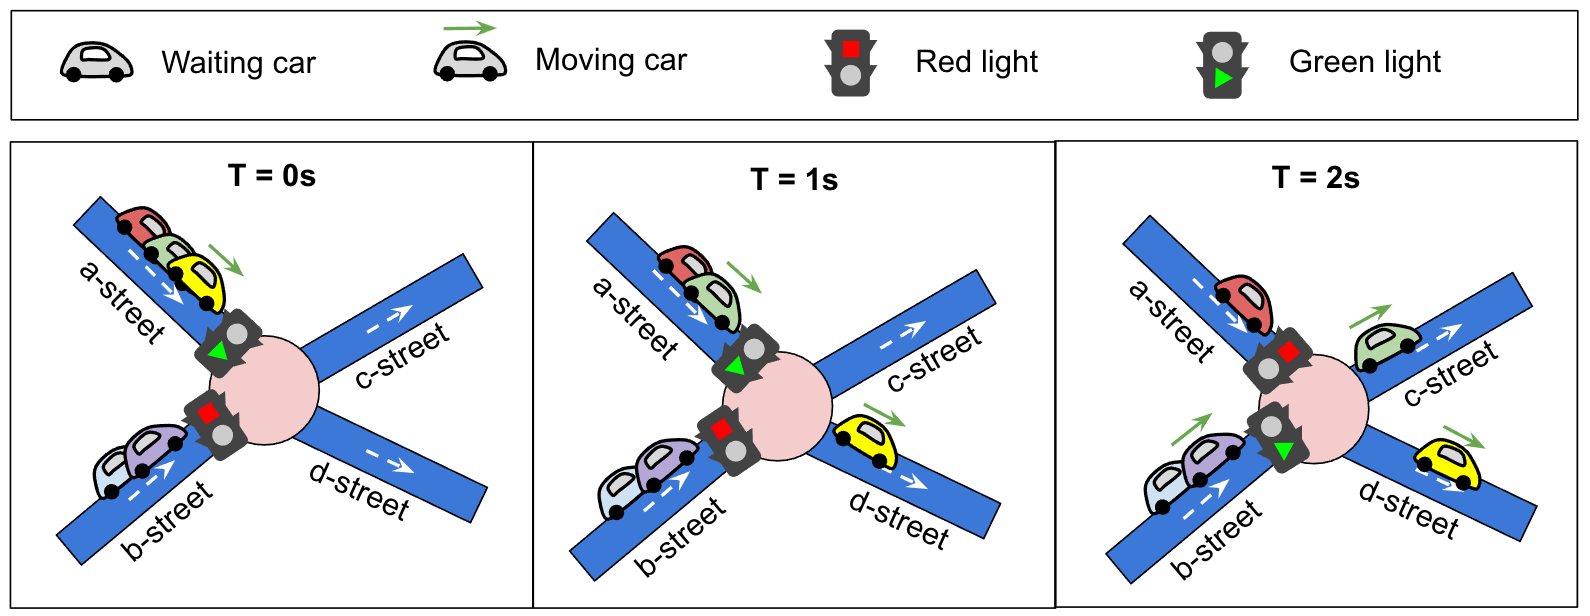
\includegraphics[width=.8\linewidth]{img/hashcode/figure2-abc.png}
    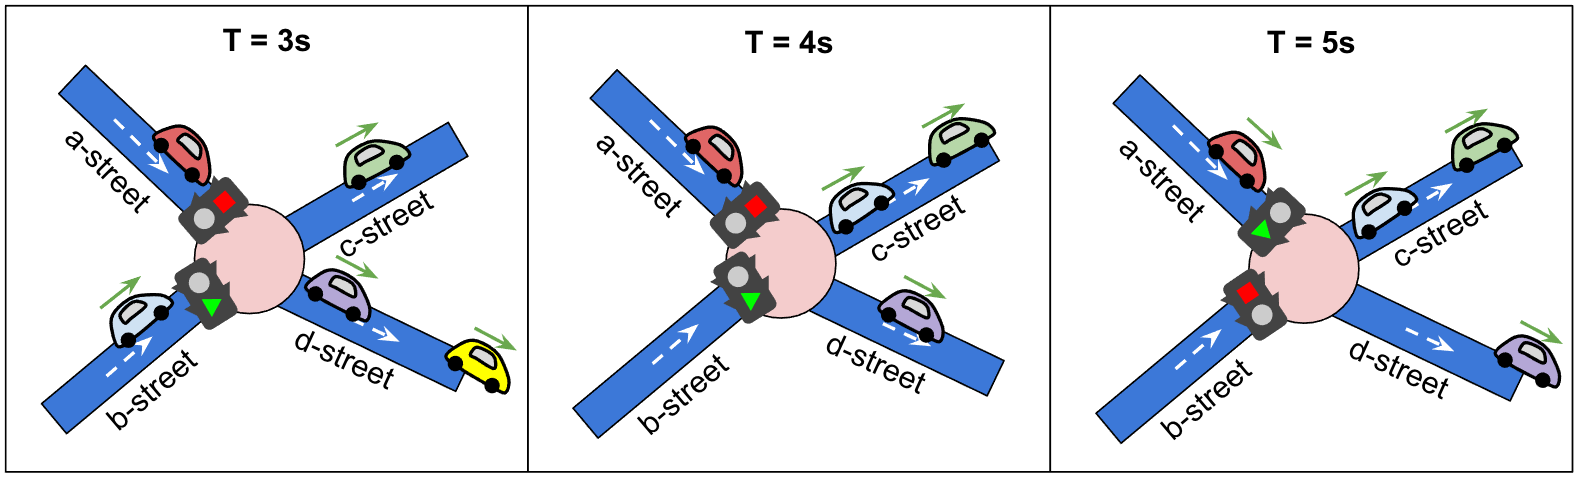
\includegraphics[width=\linewidth]{img/hashcode/figure2-def.png}
    % 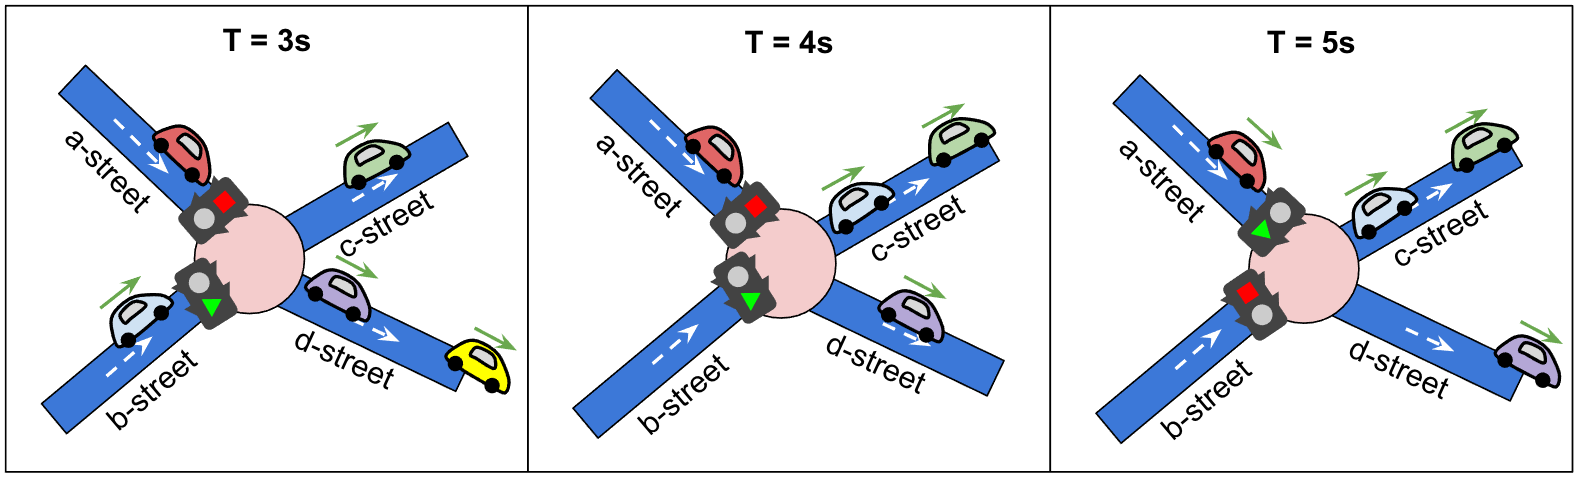
\includegraphics[width=.8\linewidth]{img/hashcode/figure2-def.png}
    \caption[Example of a traffic light schedule]{
        This figure shows how the traffic light schedule works for an intersection with two incoming streets \cite{google_coding_competitions}.
        The schedule is as follows: first \textit{a-street} for $2$ seconds, then \textit{b-street} for $3$ seconds.
        We can see the first two cars from \textit{a-street} pass in the first two seconds, then the green light switches to \textit{b-street} for three seconds,
        allowing the two cars from \textit{b-street} pass. The last car from \textit{a-street} waits till the beginning of the next cycle and then passes.
    }
    \label{fig:hashcode_traffic_lights}
\end{figure}

\subsection{Cars}

Furthermore, we have a set of cars $C$, where $1 \leq \abs{C} \leq 10^3$. Each car $c \in C$ has a given path through the city. The path is a sequence of streets the car has to drive through. The number of streets in the path is limited: $\forall c \in C \;\; 2 \leq \abs{\bm{p_c}} \leq 10^3$. No intersection or street can be repeated in the path.

At the beginning of the simulation, all cars are at the end of the first street in their path. They either wait if the light is red or are ready to move if the light is green. If more cars start at the end of the same street, they queue up in a predetermined order (See Figure~\ref{fig:hashcode_street}). When a car reaches the end of the last street in its path, it is immediately removed from the street.

\begin{figure}[ht] % h = here, t = top, p = page of floats
    \centering
    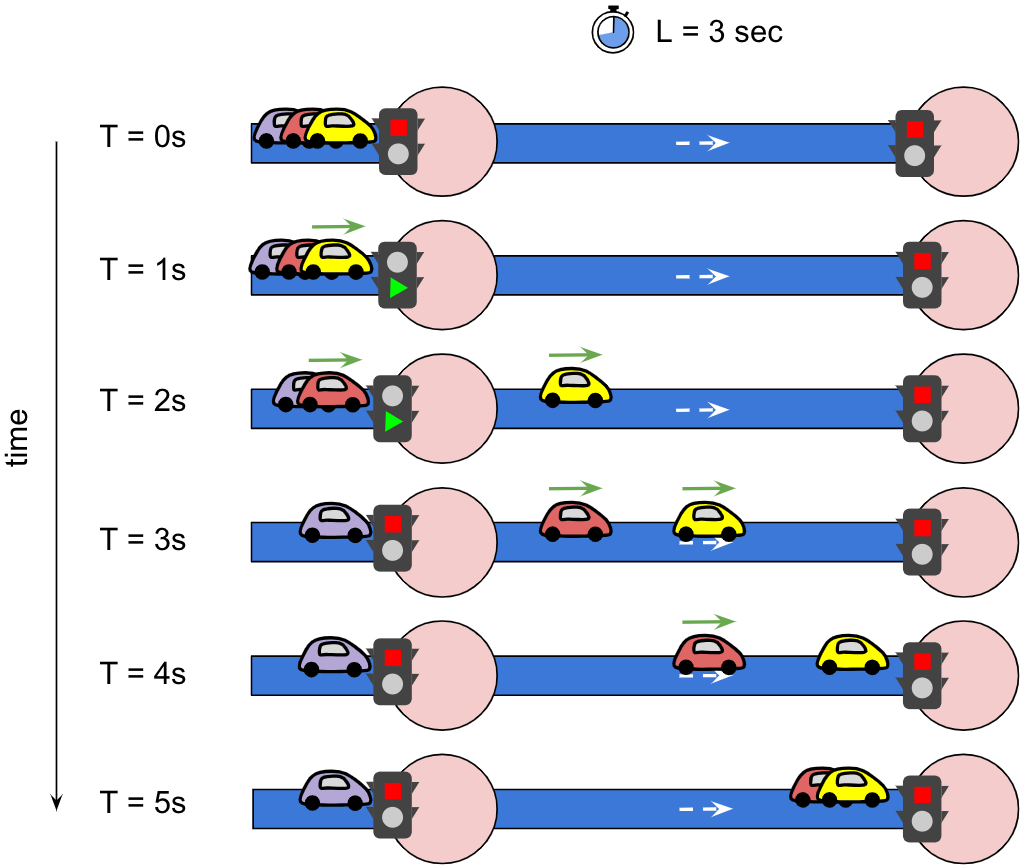
\includegraphics[width=\linewidth]{img/hashcode/figure3.png}
    %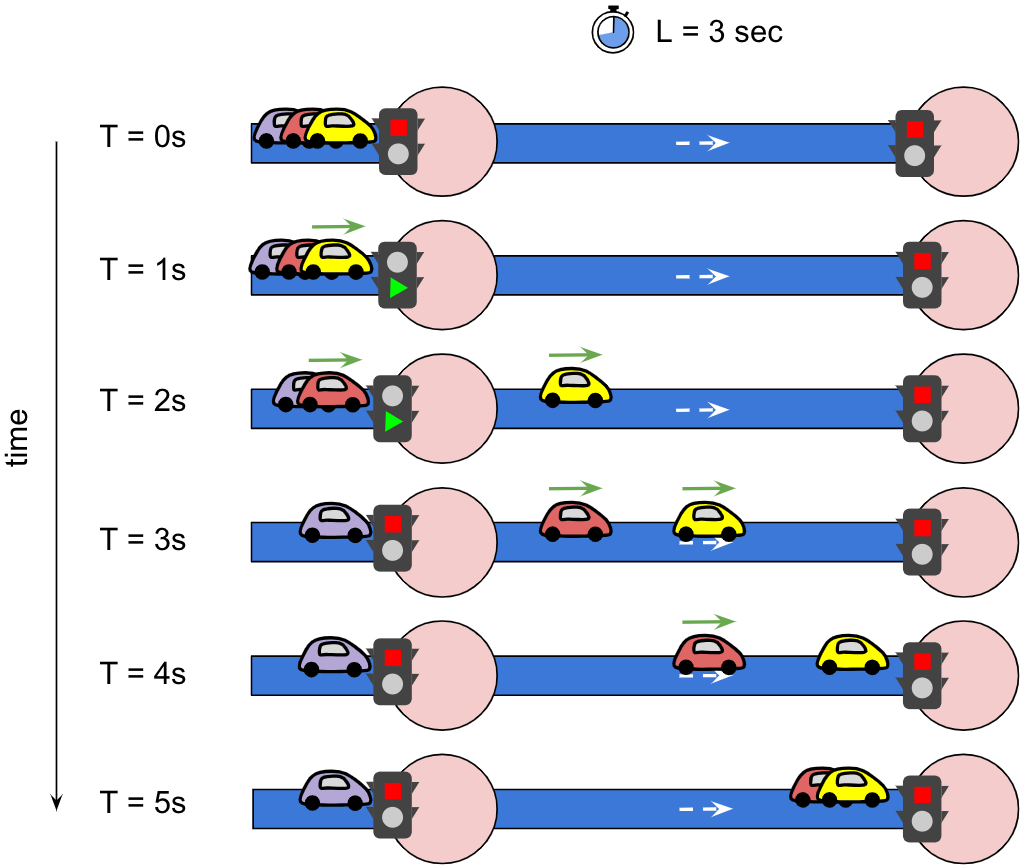
\includegraphics[width=.8\linewidth]{img/hashcode/figure3.png}
    \caption[Example of cars driving through a street]{
        This figure shows the first five seconds of a~simulation \cite{google_coding_competitions}.
        For simplicity, only one street is shown in the figure; when the light is red for this street, it is green for another street in the same intersection.
        When the light turns green at $T=1s$, the first (yellow) car immediately passes the intersection and moves to the next street, reaching the end of the street at $T=4s$.
        At $T=2s$, the light is still green, so the second (red) car passes the intersection and moves to the next street, reaching the end of the street at $T=5s$.
        From $T=3s$ to $T=5s$, the light is red, so the third (purple) car cannot pass the intersection and has to wait for the next cycle.
    }
    \label{fig:hashcode_street}
\end{figure}

\newpage

\subsection{Score}

The score of a solution is determined as follows: Let $\bm{\theta}$ denote the traffic light schedule. Given a duration of the simulation $\mathrm{D}$ in seconds, where $1 \leq \mathrm{D} \leq 10^4$, and a fixed bonus for reaching the destination $\mathrm{F}$, where $1 \leq \mathrm{F} \leq 10^3$, let $t(c; \bm{\theta}) \in \mathbb{N}$ be the time a car $c \in C$ reaches the destination. The $score$ of a car $c$ is defined as

\begin{equation}
    score(c; \bm{\theta}) =
    \begin{cases}
        \mathrm{F} + (\mathrm{D} - t(c; \bm{\theta})), & \text{if $t(c; \bm{\theta}) \leq \mathrm{D}$}, \\
        0, & \text{otherwise}.
    \end{cases}
\end{equation}

The $SCORE$ of a solution $\bm{\theta}$ is defined as

\begin{equation}
    SCORE(\bm{\theta}) = \sum_{c \in C} score(c; \bm{\theta}).
\end{equation}
